\documentclass{article}

\usepackage{ctex}
\usepackage[left=1.25in,right=1.25in,top=1in,bottom=1in]{geometry}
\usepackage{amsmath}
\usepackage{amssymb}
\usepackage{graphicx}
\usepackage{listings}
\lstset{language=Matlab}   
\lstset{breaklines}              
\lstset{extendedchars=false}
\usepackage[framed,numbered,autolinebreaks,useliterate]{mcode}

\author{张泽宇}
\date{2022年3月20日}
\title{第四周工作总结}

\begin{document}
	\maketitle
	{\centering \rule[15pt]{15cm}{0.1em}}
	
	{
		\noindent
		\large
		\textbf{这一周的主要进行的工作包括有:
			\begin{itemize}
				\item 对上周提到的三相电路模型进行了学习,掌握了simulink中相关的模块使用方法。
				\item 阅读《电力系统分析》,对三相电路故障进行了学习。
				\item 从故障电阻的位置和三相故障的种类出发仿真模拟得出数据集。
				\item 对自动调节simulink中电阻阻值设定进行了探索。
				\item 搭建了一个模拟输电配电的电路,但故障仿真时出现预期之外的问题,仍需调整。
			\end{itemize}
		}
	
	以下为详细叙述
	
	{\centering \rule[-10pt]{15cm}{0.1em}}
	
	\section{简单三相电路模型学习}
	
	如图,在这个简单的三相电路模型中,三相电压由Three-Phase Source模块提供,其中可以设置联结方式(Configuration),有三种联结方法:
	Y:星形连接中性点不接地;
	Yn:星形连接中性点经端子N引出;
	Yg:星形连接中性点接地。
	同时,也可以设定相电压值、A相的初相位等。在这个模块中已经mask了RL支路,如果采用Three-Phase Programmable Voltage Source模块,则需要再加入RL支路。
	
	Three-Phase Series RLC Load 模块提供接地负载,可以设定它的额定电压、额定频率,以及有功、无功功率等。Three-Phase V-I Measurement 模块可以测定三相电压及三相电流,信号线接口连接示波器。Distributed Parameters Line 模块模拟输电线,可以设置它的长度、频率(Frequency used for rlc specification)、以及单位长度上的电阻、电感、电容值。借助这个模块,可以实现不同位置上的故障发生模拟。
	Three-Phase Transformer (Two Windings)是最普通的一种三相变压器,可以设置它的一二侧额定电压、额定容量、联结方式等。Three-Phase Fault是故障发生装置,初始状态设置为0,则防止开始时电路正常。当进入Switching times参数设定的时间段内时,发生故障,发生的故障可以通过Fault between参数进行勾选,能够模拟四种三相故障。通过measurement选项框和万用表、示波器,可以观察得到三相故障电流和故障电压。
	
	\begin{figure}[h]
		\centering
		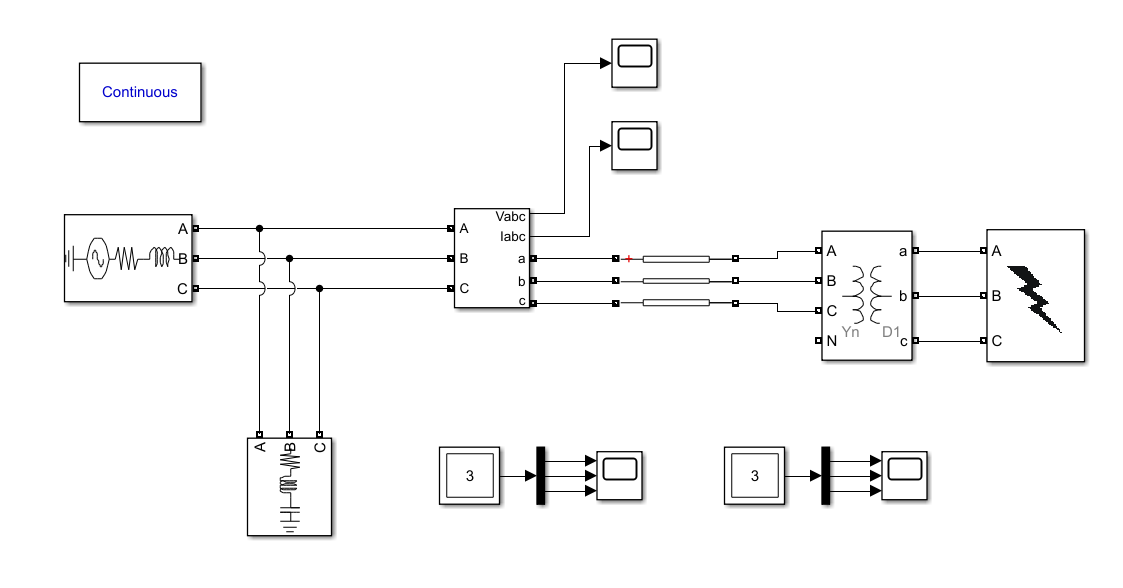
\includegraphics[width=11cm]{figure/three_phase.png}
		\caption{简单三相电路}
	\end{figure}
	总而言之,通过simulink提供的这个库,可以方便的实现三相电路的仿真。
	
	\section{三相故障}
	
	电力系统中存在有短路、断路以及各种复杂的故障。对电力系统影响最大的是短路。故障分析重点是对短路故障的分析。由于电力系统中,除了中性点以外,相与相、相与地之间都是绝缘的,因此所谓的短路是指相与相或者相与地之间发生短接。
	
	简单的短路故障有四种类型:
	
	\begin{enumerate}
		\item 三相短路
		\item 单相短路接地
		\item 两相短路
		\item 两相短路接地
	\end{enumerate}

	其中,三相短路是对称的,对电力系统的影响最大;单相短路接地最容易发生,概率可达60\%;对于除三相短路的其他非对称故障,可以采用对称分量法进行分析。
	
	导致短路发生的原因很多,根本原因是电气设备载流部分相与相或者相与地之间的绝缘遭到破坏。
	
	在短路之后,对电气设备和电力系统的正常运行都会造成很大的危害。
	
	\begin{itemize}
		\item 短路回路中电流急剧增加,数值可能超过额定电流的多倍。短路点与发电机的距离越近,短路电流越大。
		\item 短路点可能会形成电弧。
		\item 短路引起电网中电压降低,特别是靠近短路点处电压下降最多。
		\item 可能会引起系统失去稳定。
		\item 不对称接地短路会产生不平衡磁通。
	\end{itemize}

	短路故障主要分析故障电流、短路容量(短路电流和故障前电压的乘积)、故障后各点电压等。
	
	在短路仿真时,通常采用无限大功率电源。无限大功率电源是指电源的电压幅值和频率在故障过程中仍能保持恒定。即短路对电源造成的影响很小。
	
	\section{搭建电路进行仿真}
	
	基于上述的学习,我仿照现有的电路模型搭建了一个得出故障样本的简单三相电路。在这个电路中,用三相电源替代提供的电机模型,主要是考虑到采用无限大功率电源模型。
	
	\begin{figure}[h]
		\centering
		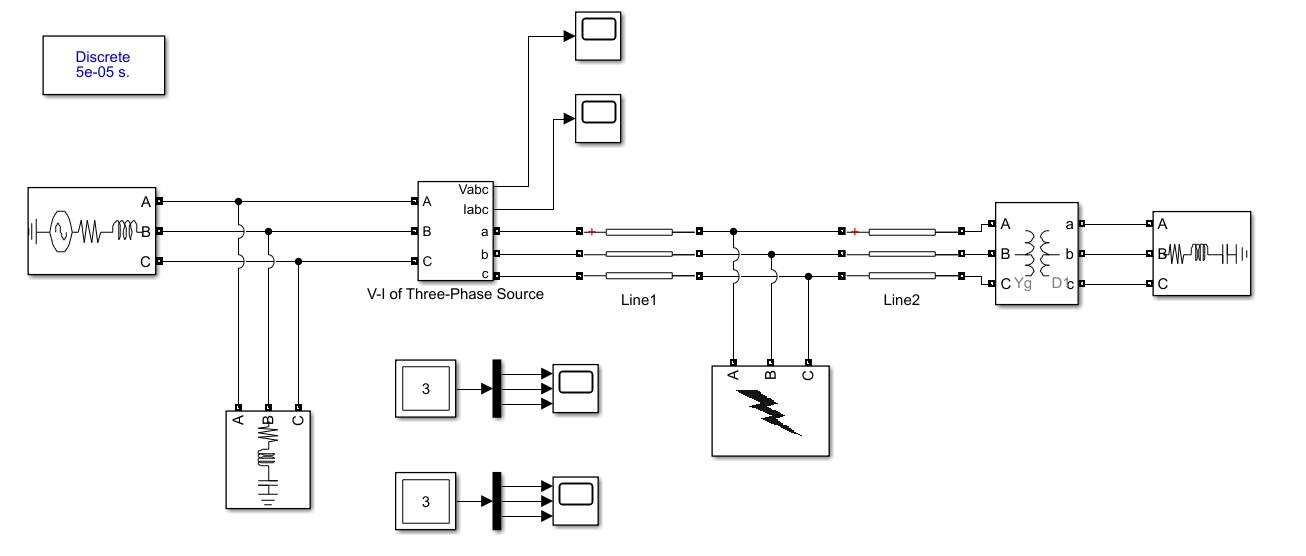
\includegraphics[width=11cm]{figure/three_phase_vary.png}
		\caption{加入故障电阻的简单三相电路}
	\end{figure}
	
	通过调整Line1和Line2的长度,在单位长度上的电阻和电感值设置相等的情况下,可以模拟不同位置电路故障的发生。假定输电线长度为200km,当Line1=100km,Line2=100km时,即为输电线中点处发生故障;当Line1=50km,Line2=150km时,即为四分之一点处发生故障。
	
	通过调整Three-Phase Fault中的故障选项,可以仿真出四种电路故障。勾选PhaseA和Ground,模拟出单相接地故障;勾选PhaseA和PhaseB,模拟两相短路故障;勾选PhaseA、PhaseB和Ground,模拟两相接地短路故障;勾选PhaseA、PhaseB、PhaseC和Ground,模拟三相接地短路故障。
	
	我以10km为间隔,将Line分为20处可能的故障点,标记为$T_{i}$,每一个故障点下仿真出正常情况和四种短路故障,得到了100张原始的数据集。
	
	\begin{figure}[h]
		\centering
		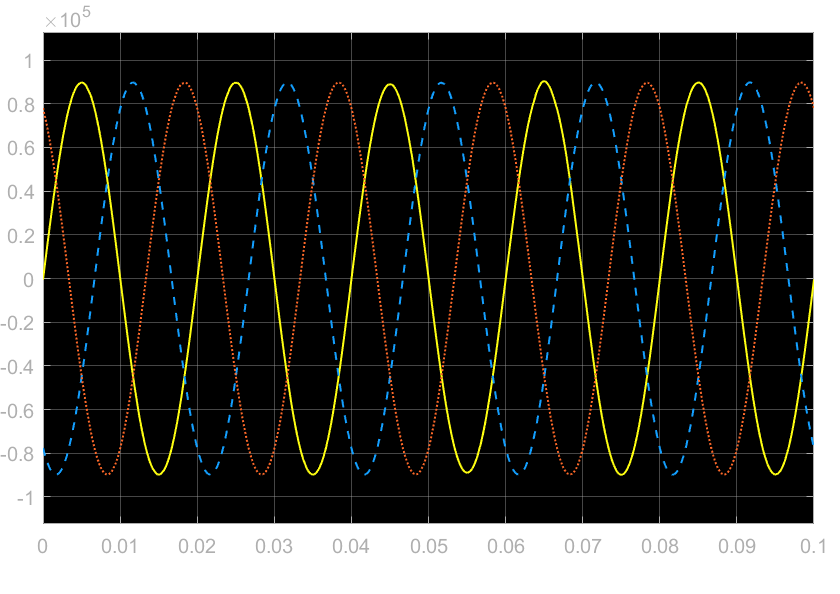
\includegraphics[width=7cm]{figure/Us.png}
		\caption{输电线中点处发生单相短路接地故障时三相电源电压波形}
	\end{figure}

	\begin{figure}[htpb]
		\centering
		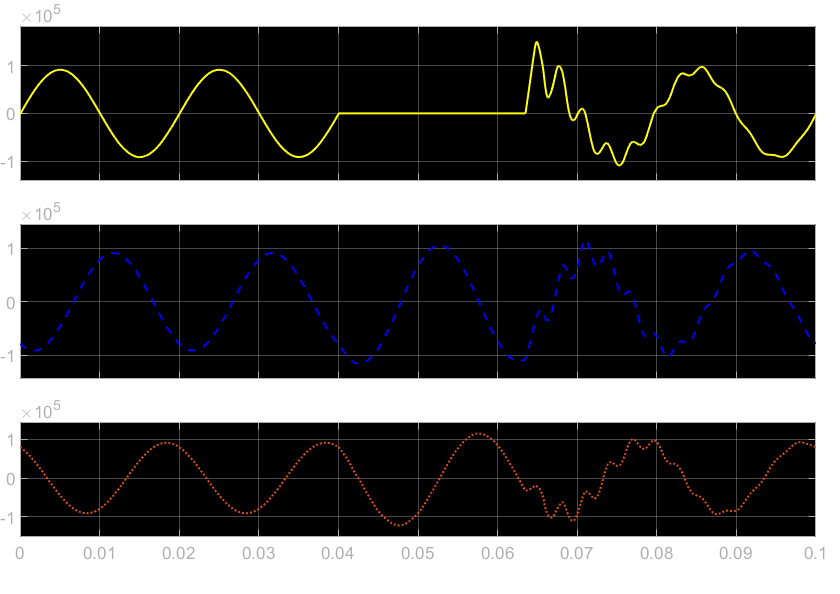
\includegraphics[width=7cm]{figure/Uf.png}
		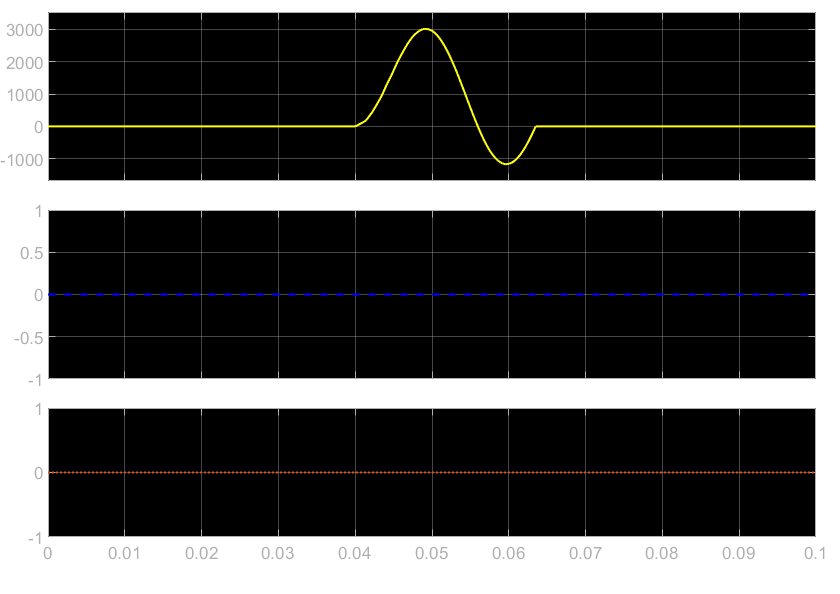
\includegraphics[width=7cm]{figure/if.png}
		\caption{输电线中点处发生单相短路接地故障时故障电压和故障电流}
	\end{figure}
	
	\section{自动调节阻值代码}
	
	针对上周所提出的需要大量改变阻值,人工操作复杂的问题,我找到了如下几种解决方法。
	
	一是改变软件,使用PSCAD而不是simulink。
	
	二是在simulink中设计GUI进行修改,但复杂程度并没有得到很好的解决。
	
	三是编写代码,构造一个电阻网络。通过循环不断地向网络中添加电阻,从而达到修改总电阻的目的。这里的技术难点在于不同于直接从simulink库浏览器中拖动原件,而是需要先绘制符号表示电阻,在把电阻的电气属性赋予这个符号。我在图书馆中查到了一种利用命令生产模型的解决的方案:
	\begin{lstlisting}
		L=7;
		M='sss1';
		new_system(M);
		open_system(M);
		for i =1:L
			i1=int2str(i);
			i0=int2str(i-1);
			pos1=[100+(i-1)*70 50 125+(i-1)*70 70];
			pos2=pos1+[25 50 25 50];
			pos3=pos1+[0 100 0 100];
			scr='f1_lib/Electrical/Electrical Elements/Resistor';
			add_block(src,[M '/ra' i1],'Position',pos1,'R',i1);
			add_block(src,[M '/rb' i1],'Position',pos2,'Orientation','down','R',i1);
			add_block(src,[M '/rc' i1],'Position',pos3,'R', i1);
			add_line(M,['ra' i1 '/RConn1'],['rb' i1 '/LConn1']);
			add_line(M,['rb' i1 '/RConn1'],['rc' i1 '/LConn1']);
			if i>1
				add_line(M,['ra' i0 '/RConn1'],['ra' i1 '/LConn1']);
				add_line(M,['rc' i0 '/RConn1'],['rc' i1 '/LConn1']);
			end
		end
	\end{lstlisting}

	在代码中,修改L的值和add\_block,可以构造出不同网络,等效成不同电阻,从而实现自动修改电阻阻值的效果。
	
	\section{模拟输电配电的电路}
	
	我自己凭借已有的知识,搭建了一个模拟输电配电的电路。
	
	\begin{figure}[h]
		\centering
		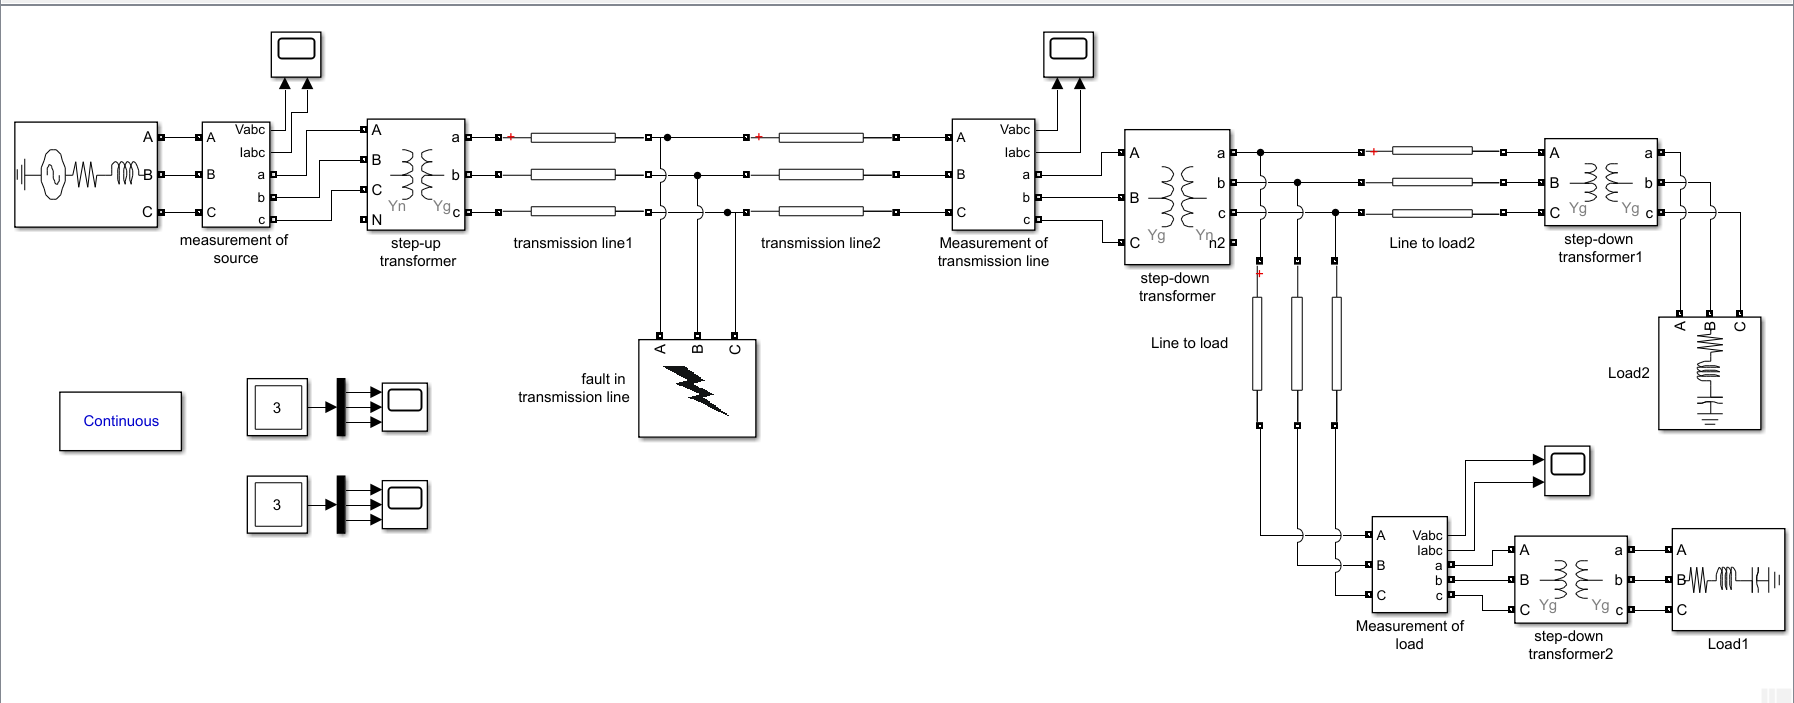
\includegraphics[width=13cm]{figure/grid.png}
		\caption{模拟输电配电的电路}
	\end{figure}

	其中三相电源发出110kv的电压,经过升压变压器升至500kv,通过全场100km的输电线,经过降压变压器降至10kv,再通过两端10km输电线接到降压变压器,降至220v,然后接到两个负载上。通过在输电线上构造故障电阻,在0.04s-0.06s模拟出不同的短路故障,用万用表显示出故障电流和故障电压,并且观察负载端的电流与电压。
	
	然而,当模拟故障时,发现故障消除之后,电路非但没有逐渐回归正常,反而表现出了类似于震荡的现象。我个人认为是因为电路中一些模块的参数设置不合理,需要进一步进行修改和调试。
\end{document}